
% Default to the notebook output style

    


% Inherit from the specified cell style.




    
\documentclass[11pt]{article}

    
    
    \usepackage[T1]{fontenc}
    % Nicer default font (+ math font) than Computer Modern for most use cases
    \usepackage{mathpazo}

    % Basic figure setup, for now with no caption control since it's done
    % automatically by Pandoc (which extracts ![](path) syntax from Markdown).
    \usepackage{graphicx}
    % We will generate all images so they have a width \maxwidth. This means
    % that they will get their normal width if they fit onto the page, but
    % are scaled down if they would overflow the margins.
    \makeatletter
    \def\maxwidth{\ifdim\Gin@nat@width>\linewidth\linewidth
    \else\Gin@nat@width\fi}
    \makeatother
    \let\Oldincludegraphics\includegraphics
    % Set max figure width to be 80% of text width, for now hardcoded.
    \renewcommand{\includegraphics}[1]{\Oldincludegraphics[width=.8\maxwidth]{#1}}
    % Ensure that by default, figures have no caption (until we provide a
    % proper Figure object with a Caption API and a way to capture that
    % in the conversion process - todo).
    \usepackage{caption}
    \DeclareCaptionLabelFormat{nolabel}{}
    \captionsetup{labelformat=nolabel}

    \usepackage{adjustbox} % Used to constrain images to a maximum size 
    \usepackage{xcolor} % Allow colors to be defined
    \usepackage{enumerate} % Needed for markdown enumerations to work
    \usepackage{geometry} % Used to adjust the document margins
    \usepackage{amsmath} % Equations
    \usepackage{amssymb} % Equations
    \usepackage{textcomp} % defines textquotesingle
    % Hack from http://tex.stackexchange.com/a/47451/13684:
    \AtBeginDocument{%
        \def\PYZsq{\textquotesingle}% Upright quotes in Pygmentized code
    }
    \usepackage{upquote} % Upright quotes for verbatim code
    \usepackage{eurosym} % defines \euro
    \usepackage[mathletters]{ucs} % Extended unicode (utf-8) support
    \usepackage[utf8x]{inputenc} % Allow utf-8 characters in the tex document
    \usepackage{fancyvrb} % verbatim replacement that allows latex
    \usepackage{grffile} % extends the file name processing of package graphics 
                         % to support a larger range 
    % The hyperref package gives us a pdf with properly built
    % internal navigation ('pdf bookmarks' for the table of contents,
    % internal cross-reference links, web links for URLs, etc.)
    \usepackage{hyperref}
    \usepackage{longtable} % longtable support required by pandoc >1.10
    \usepackage{booktabs}  % table support for pandoc > 1.12.2
    \usepackage[inline]{enumitem} % IRkernel/repr support (it uses the enumerate* environment)
    \usepackage[normalem]{ulem} % ulem is needed to support strikethroughs (\sout)
                                % normalem makes italics be italics, not underlines
    

    
    
    % Colors for the hyperref package
    \definecolor{urlcolor}{rgb}{0,.145,.698}
    \definecolor{linkcolor}{rgb}{.71,0.21,0.01}
    \definecolor{citecolor}{rgb}{.12,.54,.11}

    % ANSI colors
    \definecolor{ansi-black}{HTML}{3E424D}
    \definecolor{ansi-black-intense}{HTML}{282C36}
    \definecolor{ansi-red}{HTML}{E75C58}
    \definecolor{ansi-red-intense}{HTML}{B22B31}
    \definecolor{ansi-green}{HTML}{00A250}
    \definecolor{ansi-green-intense}{HTML}{007427}
    \definecolor{ansi-yellow}{HTML}{DDB62B}
    \definecolor{ansi-yellow-intense}{HTML}{B27D12}
    \definecolor{ansi-blue}{HTML}{208FFB}
    \definecolor{ansi-blue-intense}{HTML}{0065CA}
    \definecolor{ansi-magenta}{HTML}{D160C4}
    \definecolor{ansi-magenta-intense}{HTML}{A03196}
    \definecolor{ansi-cyan}{HTML}{60C6C8}
    \definecolor{ansi-cyan-intense}{HTML}{258F8F}
    \definecolor{ansi-white}{HTML}{C5C1B4}
    \definecolor{ansi-white-intense}{HTML}{A1A6B2}

    % commands and environments needed by pandoc snippets
    % extracted from the output of `pandoc -s`
    \providecommand{\tightlist}{%
      \setlength{\itemsep}{0pt}\setlength{\parskip}{0pt}}
    \DefineVerbatimEnvironment{Highlighting}{Verbatim}{commandchars=\\\{\}}
    % Add ',fontsize=\small' for more characters per line
    \newenvironment{Shaded}{}{}
    \newcommand{\KeywordTok}[1]{\textcolor[rgb]{0.00,0.44,0.13}{\textbf{{#1}}}}
    \newcommand{\DataTypeTok}[1]{\textcolor[rgb]{0.56,0.13,0.00}{{#1}}}
    \newcommand{\DecValTok}[1]{\textcolor[rgb]{0.25,0.63,0.44}{{#1}}}
    \newcommand{\BaseNTok}[1]{\textcolor[rgb]{0.25,0.63,0.44}{{#1}}}
    \newcommand{\FloatTok}[1]{\textcolor[rgb]{0.25,0.63,0.44}{{#1}}}
    \newcommand{\CharTok}[1]{\textcolor[rgb]{0.25,0.44,0.63}{{#1}}}
    \newcommand{\StringTok}[1]{\textcolor[rgb]{0.25,0.44,0.63}{{#1}}}
    \newcommand{\CommentTok}[1]{\textcolor[rgb]{0.38,0.63,0.69}{\textit{{#1}}}}
    \newcommand{\OtherTok}[1]{\textcolor[rgb]{0.00,0.44,0.13}{{#1}}}
    \newcommand{\AlertTok}[1]{\textcolor[rgb]{1.00,0.00,0.00}{\textbf{{#1}}}}
    \newcommand{\FunctionTok}[1]{\textcolor[rgb]{0.02,0.16,0.49}{{#1}}}
    \newcommand{\RegionMarkerTok}[1]{{#1}}
    \newcommand{\ErrorTok}[1]{\textcolor[rgb]{1.00,0.00,0.00}{\textbf{{#1}}}}
    \newcommand{\NormalTok}[1]{{#1}}
    
    % Additional commands for more recent versions of Pandoc
    \newcommand{\ConstantTok}[1]{\textcolor[rgb]{0.53,0.00,0.00}{{#1}}}
    \newcommand{\SpecialCharTok}[1]{\textcolor[rgb]{0.25,0.44,0.63}{{#1}}}
    \newcommand{\VerbatimStringTok}[1]{\textcolor[rgb]{0.25,0.44,0.63}{{#1}}}
    \newcommand{\SpecialStringTok}[1]{\textcolor[rgb]{0.73,0.40,0.53}{{#1}}}
    \newcommand{\ImportTok}[1]{{#1}}
    \newcommand{\DocumentationTok}[1]{\textcolor[rgb]{0.73,0.13,0.13}{\textit{{#1}}}}
    \newcommand{\AnnotationTok}[1]{\textcolor[rgb]{0.38,0.63,0.69}{\textbf{\textit{{#1}}}}}
    \newcommand{\CommentVarTok}[1]{\textcolor[rgb]{0.38,0.63,0.69}{\textbf{\textit{{#1}}}}}
    \newcommand{\VariableTok}[1]{\textcolor[rgb]{0.10,0.09,0.49}{{#1}}}
    \newcommand{\ControlFlowTok}[1]{\textcolor[rgb]{0.00,0.44,0.13}{\textbf{{#1}}}}
    \newcommand{\OperatorTok}[1]{\textcolor[rgb]{0.40,0.40,0.40}{{#1}}}
    \newcommand{\BuiltInTok}[1]{{#1}}
    \newcommand{\ExtensionTok}[1]{{#1}}
    \newcommand{\PreprocessorTok}[1]{\textcolor[rgb]{0.74,0.48,0.00}{{#1}}}
    \newcommand{\AttributeTok}[1]{\textcolor[rgb]{0.49,0.56,0.16}{{#1}}}
    \newcommand{\InformationTok}[1]{\textcolor[rgb]{0.38,0.63,0.69}{\textbf{\textit{{#1}}}}}
    \newcommand{\WarningTok}[1]{\textcolor[rgb]{0.38,0.63,0.69}{\textbf{\textit{{#1}}}}}
    
    
    % Define a nice break command that doesn't care if a line doesn't already
    % exist.
    \def\br{\hspace*{\fill} \\* }
    % Math Jax compatability definitions
    \def\gt{>}
    \def\lt{<}
    % Document parameters
    \title{Project Writeup}
    
    
    

    % Pygments definitions
    
\makeatletter
\def\PY@reset{\let\PY@it=\relax \let\PY@bf=\relax%
    \let\PY@ul=\relax \let\PY@tc=\relax%
    \let\PY@bc=\relax \let\PY@ff=\relax}
\def\PY@tok#1{\csname PY@tok@#1\endcsname}
\def\PY@toks#1+{\ifx\relax#1\empty\else%
    \PY@tok{#1}\expandafter\PY@toks\fi}
\def\PY@do#1{\PY@bc{\PY@tc{\PY@ul{%
    \PY@it{\PY@bf{\PY@ff{#1}}}}}}}
\def\PY#1#2{\PY@reset\PY@toks#1+\relax+\PY@do{#2}}

\expandafter\def\csname PY@tok@w\endcsname{\def\PY@tc##1{\textcolor[rgb]{0.73,0.73,0.73}{##1}}}
\expandafter\def\csname PY@tok@c\endcsname{\let\PY@it=\textit\def\PY@tc##1{\textcolor[rgb]{0.25,0.50,0.50}{##1}}}
\expandafter\def\csname PY@tok@cp\endcsname{\def\PY@tc##1{\textcolor[rgb]{0.74,0.48,0.00}{##1}}}
\expandafter\def\csname PY@tok@k\endcsname{\let\PY@bf=\textbf\def\PY@tc##1{\textcolor[rgb]{0.00,0.50,0.00}{##1}}}
\expandafter\def\csname PY@tok@kp\endcsname{\def\PY@tc##1{\textcolor[rgb]{0.00,0.50,0.00}{##1}}}
\expandafter\def\csname PY@tok@kt\endcsname{\def\PY@tc##1{\textcolor[rgb]{0.69,0.00,0.25}{##1}}}
\expandafter\def\csname PY@tok@o\endcsname{\def\PY@tc##1{\textcolor[rgb]{0.40,0.40,0.40}{##1}}}
\expandafter\def\csname PY@tok@ow\endcsname{\let\PY@bf=\textbf\def\PY@tc##1{\textcolor[rgb]{0.67,0.13,1.00}{##1}}}
\expandafter\def\csname PY@tok@nb\endcsname{\def\PY@tc##1{\textcolor[rgb]{0.00,0.50,0.00}{##1}}}
\expandafter\def\csname PY@tok@nf\endcsname{\def\PY@tc##1{\textcolor[rgb]{0.00,0.00,1.00}{##1}}}
\expandafter\def\csname PY@tok@nc\endcsname{\let\PY@bf=\textbf\def\PY@tc##1{\textcolor[rgb]{0.00,0.00,1.00}{##1}}}
\expandafter\def\csname PY@tok@nn\endcsname{\let\PY@bf=\textbf\def\PY@tc##1{\textcolor[rgb]{0.00,0.00,1.00}{##1}}}
\expandafter\def\csname PY@tok@ne\endcsname{\let\PY@bf=\textbf\def\PY@tc##1{\textcolor[rgb]{0.82,0.25,0.23}{##1}}}
\expandafter\def\csname PY@tok@nv\endcsname{\def\PY@tc##1{\textcolor[rgb]{0.10,0.09,0.49}{##1}}}
\expandafter\def\csname PY@tok@no\endcsname{\def\PY@tc##1{\textcolor[rgb]{0.53,0.00,0.00}{##1}}}
\expandafter\def\csname PY@tok@nl\endcsname{\def\PY@tc##1{\textcolor[rgb]{0.63,0.63,0.00}{##1}}}
\expandafter\def\csname PY@tok@ni\endcsname{\let\PY@bf=\textbf\def\PY@tc##1{\textcolor[rgb]{0.60,0.60,0.60}{##1}}}
\expandafter\def\csname PY@tok@na\endcsname{\def\PY@tc##1{\textcolor[rgb]{0.49,0.56,0.16}{##1}}}
\expandafter\def\csname PY@tok@nt\endcsname{\let\PY@bf=\textbf\def\PY@tc##1{\textcolor[rgb]{0.00,0.50,0.00}{##1}}}
\expandafter\def\csname PY@tok@nd\endcsname{\def\PY@tc##1{\textcolor[rgb]{0.67,0.13,1.00}{##1}}}
\expandafter\def\csname PY@tok@s\endcsname{\def\PY@tc##1{\textcolor[rgb]{0.73,0.13,0.13}{##1}}}
\expandafter\def\csname PY@tok@sd\endcsname{\let\PY@it=\textit\def\PY@tc##1{\textcolor[rgb]{0.73,0.13,0.13}{##1}}}
\expandafter\def\csname PY@tok@si\endcsname{\let\PY@bf=\textbf\def\PY@tc##1{\textcolor[rgb]{0.73,0.40,0.53}{##1}}}
\expandafter\def\csname PY@tok@se\endcsname{\let\PY@bf=\textbf\def\PY@tc##1{\textcolor[rgb]{0.73,0.40,0.13}{##1}}}
\expandafter\def\csname PY@tok@sr\endcsname{\def\PY@tc##1{\textcolor[rgb]{0.73,0.40,0.53}{##1}}}
\expandafter\def\csname PY@tok@ss\endcsname{\def\PY@tc##1{\textcolor[rgb]{0.10,0.09,0.49}{##1}}}
\expandafter\def\csname PY@tok@sx\endcsname{\def\PY@tc##1{\textcolor[rgb]{0.00,0.50,0.00}{##1}}}
\expandafter\def\csname PY@tok@m\endcsname{\def\PY@tc##1{\textcolor[rgb]{0.40,0.40,0.40}{##1}}}
\expandafter\def\csname PY@tok@gh\endcsname{\let\PY@bf=\textbf\def\PY@tc##1{\textcolor[rgb]{0.00,0.00,0.50}{##1}}}
\expandafter\def\csname PY@tok@gu\endcsname{\let\PY@bf=\textbf\def\PY@tc##1{\textcolor[rgb]{0.50,0.00,0.50}{##1}}}
\expandafter\def\csname PY@tok@gd\endcsname{\def\PY@tc##1{\textcolor[rgb]{0.63,0.00,0.00}{##1}}}
\expandafter\def\csname PY@tok@gi\endcsname{\def\PY@tc##1{\textcolor[rgb]{0.00,0.63,0.00}{##1}}}
\expandafter\def\csname PY@tok@gr\endcsname{\def\PY@tc##1{\textcolor[rgb]{1.00,0.00,0.00}{##1}}}
\expandafter\def\csname PY@tok@ge\endcsname{\let\PY@it=\textit}
\expandafter\def\csname PY@tok@gs\endcsname{\let\PY@bf=\textbf}
\expandafter\def\csname PY@tok@gp\endcsname{\let\PY@bf=\textbf\def\PY@tc##1{\textcolor[rgb]{0.00,0.00,0.50}{##1}}}
\expandafter\def\csname PY@tok@go\endcsname{\def\PY@tc##1{\textcolor[rgb]{0.53,0.53,0.53}{##1}}}
\expandafter\def\csname PY@tok@gt\endcsname{\def\PY@tc##1{\textcolor[rgb]{0.00,0.27,0.87}{##1}}}
\expandafter\def\csname PY@tok@err\endcsname{\def\PY@bc##1{\setlength{\fboxsep}{0pt}\fcolorbox[rgb]{1.00,0.00,0.00}{1,1,1}{\strut ##1}}}
\expandafter\def\csname PY@tok@kc\endcsname{\let\PY@bf=\textbf\def\PY@tc##1{\textcolor[rgb]{0.00,0.50,0.00}{##1}}}
\expandafter\def\csname PY@tok@kd\endcsname{\let\PY@bf=\textbf\def\PY@tc##1{\textcolor[rgb]{0.00,0.50,0.00}{##1}}}
\expandafter\def\csname PY@tok@kn\endcsname{\let\PY@bf=\textbf\def\PY@tc##1{\textcolor[rgb]{0.00,0.50,0.00}{##1}}}
\expandafter\def\csname PY@tok@kr\endcsname{\let\PY@bf=\textbf\def\PY@tc##1{\textcolor[rgb]{0.00,0.50,0.00}{##1}}}
\expandafter\def\csname PY@tok@bp\endcsname{\def\PY@tc##1{\textcolor[rgb]{0.00,0.50,0.00}{##1}}}
\expandafter\def\csname PY@tok@fm\endcsname{\def\PY@tc##1{\textcolor[rgb]{0.00,0.00,1.00}{##1}}}
\expandafter\def\csname PY@tok@vc\endcsname{\def\PY@tc##1{\textcolor[rgb]{0.10,0.09,0.49}{##1}}}
\expandafter\def\csname PY@tok@vg\endcsname{\def\PY@tc##1{\textcolor[rgb]{0.10,0.09,0.49}{##1}}}
\expandafter\def\csname PY@tok@vi\endcsname{\def\PY@tc##1{\textcolor[rgb]{0.10,0.09,0.49}{##1}}}
\expandafter\def\csname PY@tok@vm\endcsname{\def\PY@tc##1{\textcolor[rgb]{0.10,0.09,0.49}{##1}}}
\expandafter\def\csname PY@tok@sa\endcsname{\def\PY@tc##1{\textcolor[rgb]{0.73,0.13,0.13}{##1}}}
\expandafter\def\csname PY@tok@sb\endcsname{\def\PY@tc##1{\textcolor[rgb]{0.73,0.13,0.13}{##1}}}
\expandafter\def\csname PY@tok@sc\endcsname{\def\PY@tc##1{\textcolor[rgb]{0.73,0.13,0.13}{##1}}}
\expandafter\def\csname PY@tok@dl\endcsname{\def\PY@tc##1{\textcolor[rgb]{0.73,0.13,0.13}{##1}}}
\expandafter\def\csname PY@tok@s2\endcsname{\def\PY@tc##1{\textcolor[rgb]{0.73,0.13,0.13}{##1}}}
\expandafter\def\csname PY@tok@sh\endcsname{\def\PY@tc##1{\textcolor[rgb]{0.73,0.13,0.13}{##1}}}
\expandafter\def\csname PY@tok@s1\endcsname{\def\PY@tc##1{\textcolor[rgb]{0.73,0.13,0.13}{##1}}}
\expandafter\def\csname PY@tok@mb\endcsname{\def\PY@tc##1{\textcolor[rgb]{0.40,0.40,0.40}{##1}}}
\expandafter\def\csname PY@tok@mf\endcsname{\def\PY@tc##1{\textcolor[rgb]{0.40,0.40,0.40}{##1}}}
\expandafter\def\csname PY@tok@mh\endcsname{\def\PY@tc##1{\textcolor[rgb]{0.40,0.40,0.40}{##1}}}
\expandafter\def\csname PY@tok@mi\endcsname{\def\PY@tc##1{\textcolor[rgb]{0.40,0.40,0.40}{##1}}}
\expandafter\def\csname PY@tok@il\endcsname{\def\PY@tc##1{\textcolor[rgb]{0.40,0.40,0.40}{##1}}}
\expandafter\def\csname PY@tok@mo\endcsname{\def\PY@tc##1{\textcolor[rgb]{0.40,0.40,0.40}{##1}}}
\expandafter\def\csname PY@tok@ch\endcsname{\let\PY@it=\textit\def\PY@tc##1{\textcolor[rgb]{0.25,0.50,0.50}{##1}}}
\expandafter\def\csname PY@tok@cm\endcsname{\let\PY@it=\textit\def\PY@tc##1{\textcolor[rgb]{0.25,0.50,0.50}{##1}}}
\expandafter\def\csname PY@tok@cpf\endcsname{\let\PY@it=\textit\def\PY@tc##1{\textcolor[rgb]{0.25,0.50,0.50}{##1}}}
\expandafter\def\csname PY@tok@c1\endcsname{\let\PY@it=\textit\def\PY@tc##1{\textcolor[rgb]{0.25,0.50,0.50}{##1}}}
\expandafter\def\csname PY@tok@cs\endcsname{\let\PY@it=\textit\def\PY@tc##1{\textcolor[rgb]{0.25,0.50,0.50}{##1}}}

\def\PYZbs{\char`\\}
\def\PYZus{\char`\_}
\def\PYZob{\char`\{}
\def\PYZcb{\char`\}}
\def\PYZca{\char`\^}
\def\PYZam{\char`\&}
\def\PYZlt{\char`\<}
\def\PYZgt{\char`\>}
\def\PYZsh{\char`\#}
\def\PYZpc{\char`\%}
\def\PYZdl{\char`\$}
\def\PYZhy{\char`\-}
\def\PYZsq{\char`\'}
\def\PYZdq{\char`\"}
\def\PYZti{\char`\~}
% for compatibility with earlier versions
\def\PYZat{@}
\def\PYZlb{[}
\def\PYZrb{]}
\makeatother


    % Exact colors from NB
    \definecolor{incolor}{rgb}{0.0, 0.0, 0.5}
    \definecolor{outcolor}{rgb}{0.545, 0.0, 0.0}



    
    % Prevent overflowing lines due to hard-to-break entities
    \sloppy 
    % Setup hyperref package
    \hypersetup{
      breaklinks=true,  % so long urls are correctly broken across lines
      colorlinks=true,
      urlcolor=urlcolor,
      linkcolor=linkcolor,
      citecolor=citecolor,
      }
    % Slightly bigger margins than the latex defaults
    
    \geometry{verbose,tmargin=1in,bmargin=1in,lmargin=1in,rmargin=1in}
    
    

    \begin{document}
    
    
    \maketitle
    
    

    
    \hypertarget{project-2---advanced-lane-finding}{%
\subsection{Project 2 - Advanced Lane
Finding}\label{project-2---advanced-lane-finding}}

\hypertarget{you-can-use-this-file-as-a-template-for-your-writeup-if-you-want-to-submit-it-as-a-markdown-file-but-feel-free-to-use-some-other-method-and-submit-a-pdf-if-you-prefer.}{%
\subsubsection{You can use this file as a template for your writeup if
you want to submit it as a markdown file, but feel free to use some
other method and submit a pdf if you
prefer.}\label{you-can-use-this-file-as-a-template-for-your-writeup-if-you-want-to-submit-it-as-a-markdown-file-but-feel-free-to-use-some-other-method-and-submit-a-pdf-if-you-prefer.}}

\begin{center}\rule{0.5\linewidth}{\linethickness}\end{center}

\textbf{Advanced Lane Finding Project}

The goals / steps of this project are the following:

\begin{itemize}
\tightlist
\item
  Compute the camera calibration matrix and distortion coefficients
  given a set of chessboard images.
\item
  Apply a distortion correction to raw images.
\item
  Use color transforms, gradients, etc., to create a thresholded binary
  image.
\item
  Apply a perspective transform to rectify binary image (``birds-eye
  view'').
\item
  Detect lane pixels and fit to find the lane boundary.
\item
  Determine the curvature of the lane and vehicle position with respect
  to center.
\item
  Warp the detected lane boundaries back onto the original image.
\item
  Output visual display of the lane boundaries and numerical estimation
  of lane curvature and vehicle position.
\end{itemize}

\hypertarget{rubric-points}{%
\subsection{\texorpdfstring{\href{https://review.udacity.com/\#!/rubrics/571/view}{Rubric}
Points}{Rubric Points}}\label{rubric-points}}

\hypertarget{here-i-will-consider-the-rubric-points-individually-and-describe-how-i-addressed-each-point-in-my-implementation.}{%
\subsubsection{Here I will consider the rubric points individually and
describe how I addressed each point in my
implementation.}\label{here-i-will-consider-the-rubric-points-individually-and-describe-how-i-addressed-each-point-in-my-implementation.}}

\begin{center}\rule{0.5\linewidth}{\linethickness}\end{center}

\hypertarget{writeup-readme}{%
\subsubsection{Writeup / README}\label{writeup-readme}}

\hypertarget{provide-a-writeup-readme-that-includes-all-the-rubric-points-and-how-you-addressed-each-one.-you-can-submit-your-writeup-as-markdown-or-pdf.-here-is-a-template-writeup-for-this-project-you-can-use-as-a-guide-and-a-starting-point.}{%
\paragraph{\texorpdfstring{1. Provide a Writeup / README that includes
all the rubric points and how you addressed each one. You can submit
your writeup as markdown or pdf.
\href{https://github.com/udacity/CarND-Advanced-Lane-Lines/blob/master/writeup_template.md}{Here}
is a template writeup for this project you can use as a guide and a
starting
point.}{1. Provide a Writeup / README that includes all the rubric points and how you addressed each one. You can submit your writeup as markdown or pdf. Here is a template writeup for this project you can use as a guide and a starting point.}}\label{provide-a-writeup-readme-that-includes-all-the-rubric-points-and-how-you-addressed-each-one.-you-can-submit-your-writeup-as-markdown-or-pdf.-here-is-a-template-writeup-for-this-project-you-can-use-as-a-guide-and-a-starting-point.}}

This is it.

\hypertarget{camera-calibration}{%
\subsubsection{Camera Calibration}\label{camera-calibration}}

\hypertarget{briefly-state-how-you-computed-the-camera-matrix-and-distortion-coefficients.-provide-an-example-of-a-distortion-corrected-calibration-image.}{%
\paragraph{1. Briefly state how you computed the camera matrix and
distortion coefficients. Provide an example of a distortion corrected
calibration
image.}\label{briefly-state-how-you-computed-the-camera-matrix-and-distortion-coefficients.-provide-an-example-of-a-distortion-corrected-calibration-image.}}

The code for this step is contained in the first code cell of the
IPython notebook located in ``./Advanced Lane Finding.ipynb''.

I start by preparing ``object points'', which will be the (x, y, z)
coordinates of the chessboard corners in the world. Here I am assuming
the chessboard is fixed on the (x, y) plane at z=0, such that the object
points are the same for each calibration image. Thus, \texttt{objp} is
just a replicated array of coordinates, and \texttt{objpoints} will be
appended with a copy of it every time I successfully detect all
chessboard corners in a test image. \texttt{imgpoints} will be appended
with the (x, y) pixel position of each of the corners in the image plane
with each successful chessboard detection.

I then used the output \texttt{objpoints} and \texttt{imgpoints} to
compute the camera calibration and distortion coefficients using the
\texttt{cv2.calibrateCamera()} function. The distortion coefficients
were stored in ``calibration\_pickle.p'' so they could be used in later
portions of the code. The

In the second code cell in the notebook, I test the calibration. First,
I read the distortion coefficients from the pickle file. Then I test
using one of the checkerboard sample files (calibration1.jpg). Here are
the results: Original file:
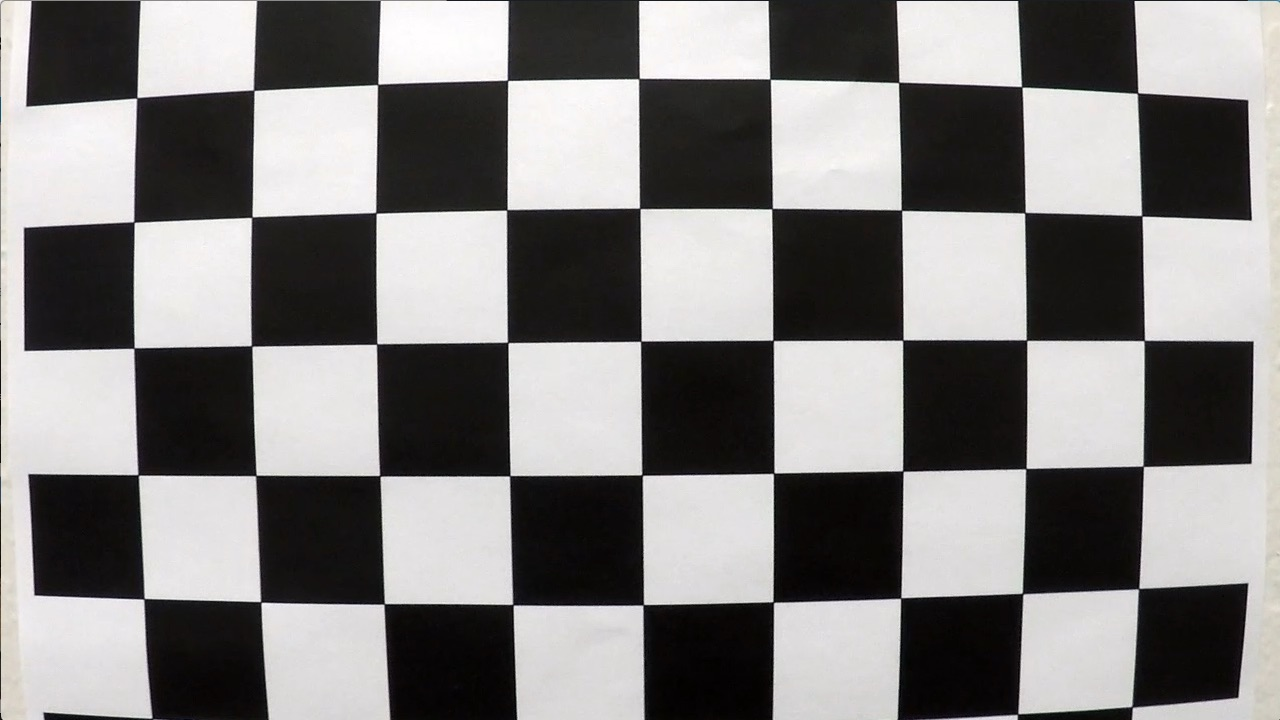
\includegraphics{./camera_cal/calibration1.jpg}

Undistorted file:
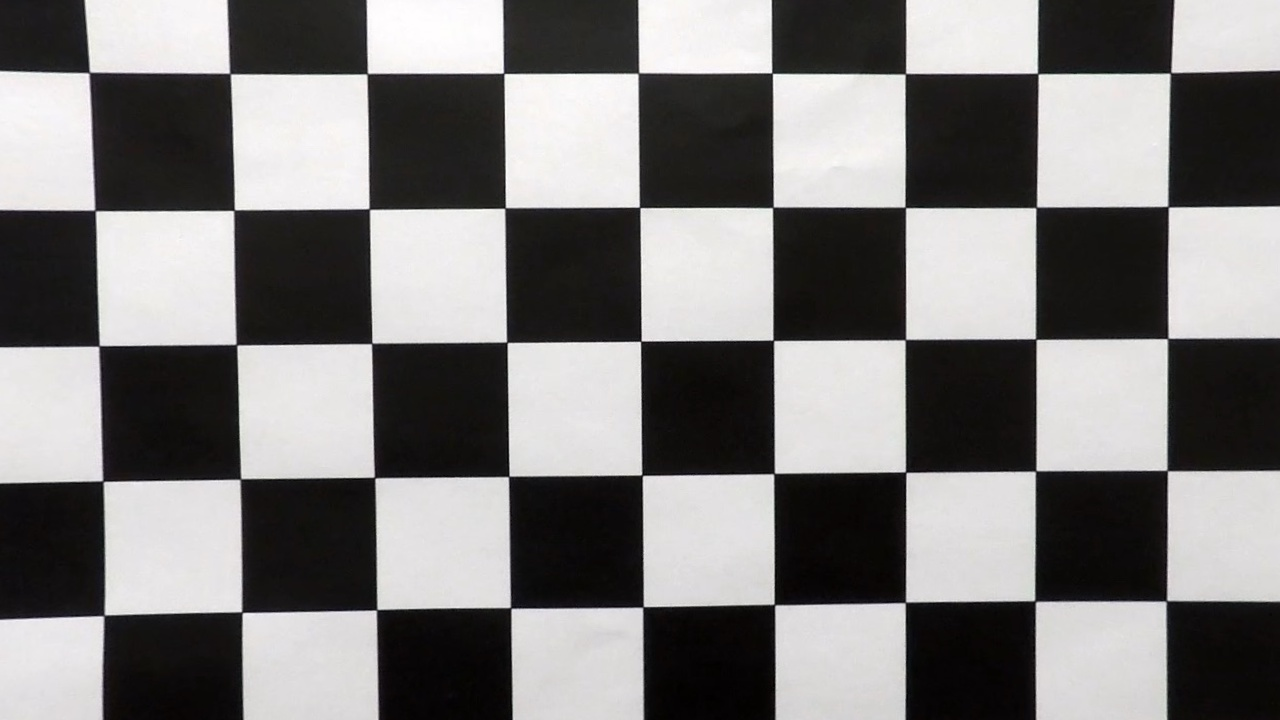
\includegraphics{./output_images/undistorted_checkerboard.jpg}

\hypertarget{pipeline-single-images}{%
\subsubsection{Pipeline (single images)}\label{pipeline-single-images}}

\hypertarget{provide-an-example-of-a-distortion-corrected-image.}{%
\paragraph{1. Provide an example of a distortion-corrected
image.}\label{provide-an-example-of-a-distortion-corrected-image.}}

In the second code cell, I also apply the same undistortion correction
to one of the sample input files. Input file:
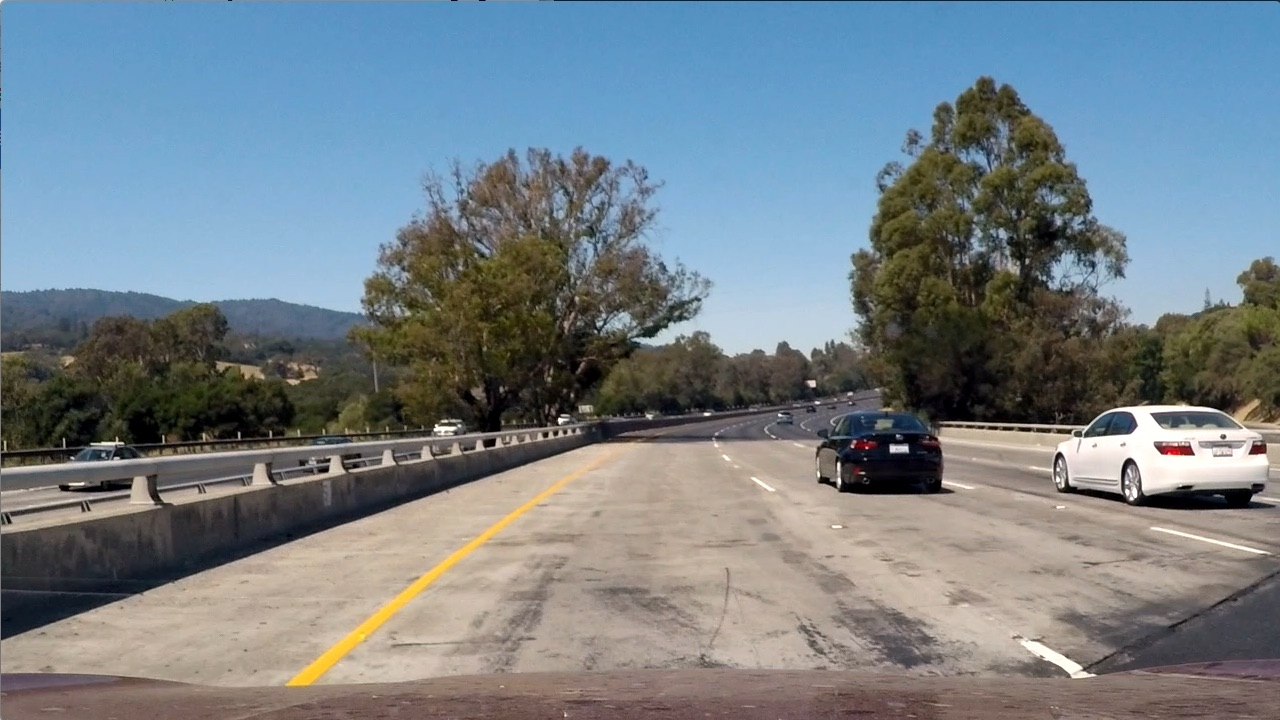
\includegraphics{./test_images/test1.jpg}

Output: 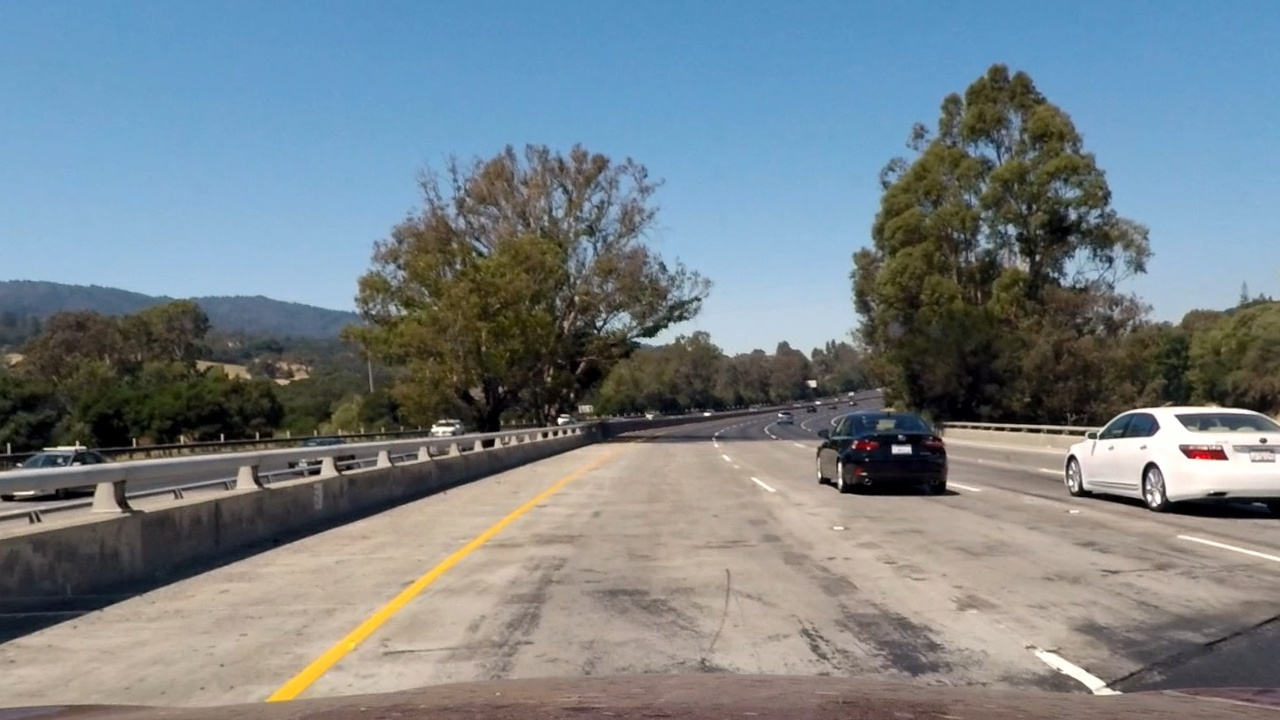
\includegraphics{./output_images/undistorted_test1.jpg}

\hypertarget{describe-how-and-identify-where-in-your-code-you-used-color-transforms-gradients-or-other-methods-to-create-a-thresholded-binary-image.-provide-an-example-of-a-binary-image-result.}{%
\paragraph{2. Describe how (and identify where in your code) you used
color transforms, gradients or other methods to create a thresholded
binary image. Provide an example of a binary image
result.}\label{describe-how-and-identify-where-in-your-code-you-used-color-transforms-gradients-or-other-methods-to-create-a-thresholded-binary-image.-provide-an-example-of-a-binary-image-result.}}

The third code cell contains a group of test code I used to eventually
build the pipeline for processing videos. While building this code cell,
images were save at every step to better understand what processing each
step was performing and how parameter adjustments affected the output.
All output files can be found in the folder ``./output\_images/''.

Functions that we created as part of the quizzes are contained in the
third code cell including sobel thresholding, magnitude thresholding,
direction thresholding, color thresholding and window masking.

The code reads each test image from ``./test\_images'', applies the
distortion coefficients and writes the file with the prefix
``undistorted\_''. Here's an example:
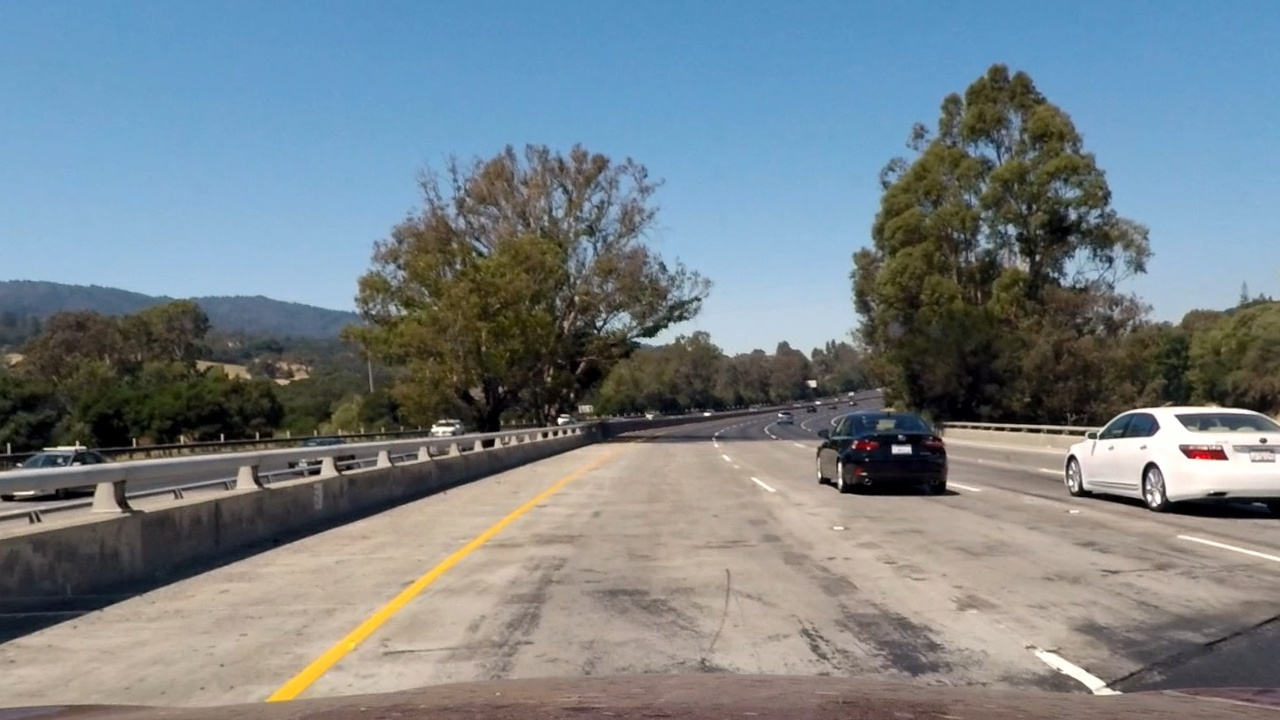
\includegraphics{./output_images/undistorted_test1.jpg}

I applied a number of the thresholding techniques to each image (sorbel
\& color, primarily) and and created combined binary threshold images.
These files were written with the prefix ``binary\_''. Here's an
example: 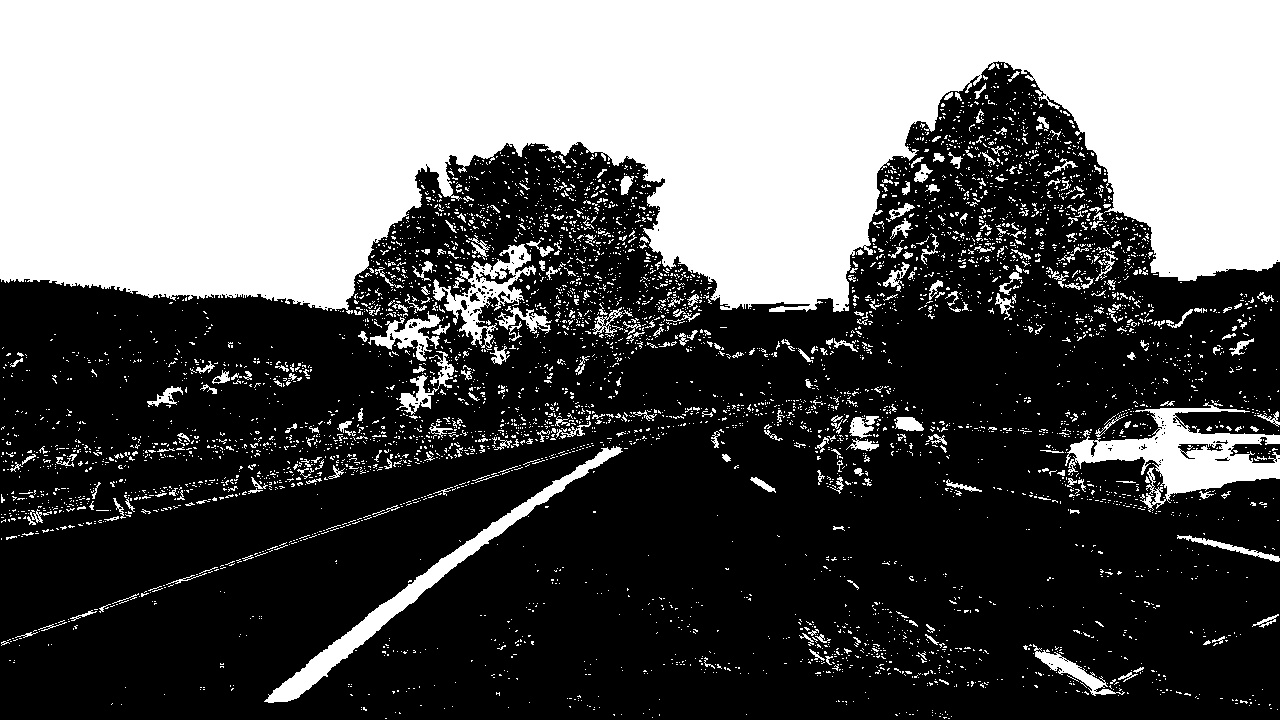
\includegraphics{./output_images/binary_test1.jpg}

\hypertarget{describe-how-and-identify-where-in-your-code-you-performed-a-perspective-transform-and-provide-an-example-of-a-transformed-image.}{%
\paragraph{3. Describe how (and identify where in your code) you
performed a perspective transform and provide an example of a
transformed
image.}\label{describe-how-and-identify-where-in-your-code-you-performed-a-perspective-transform-and-provide-an-example-of-a-transformed-image.}}

I defined a trapezoid source shape and a rectangular destination shape
and used the cv2 functions getPerspectiveTransform and warpPerspective
Transform to perform the necessary transform and generate a top
perspective of the lanes. These images were written with the prefix
``warped\_''. Here's an example:
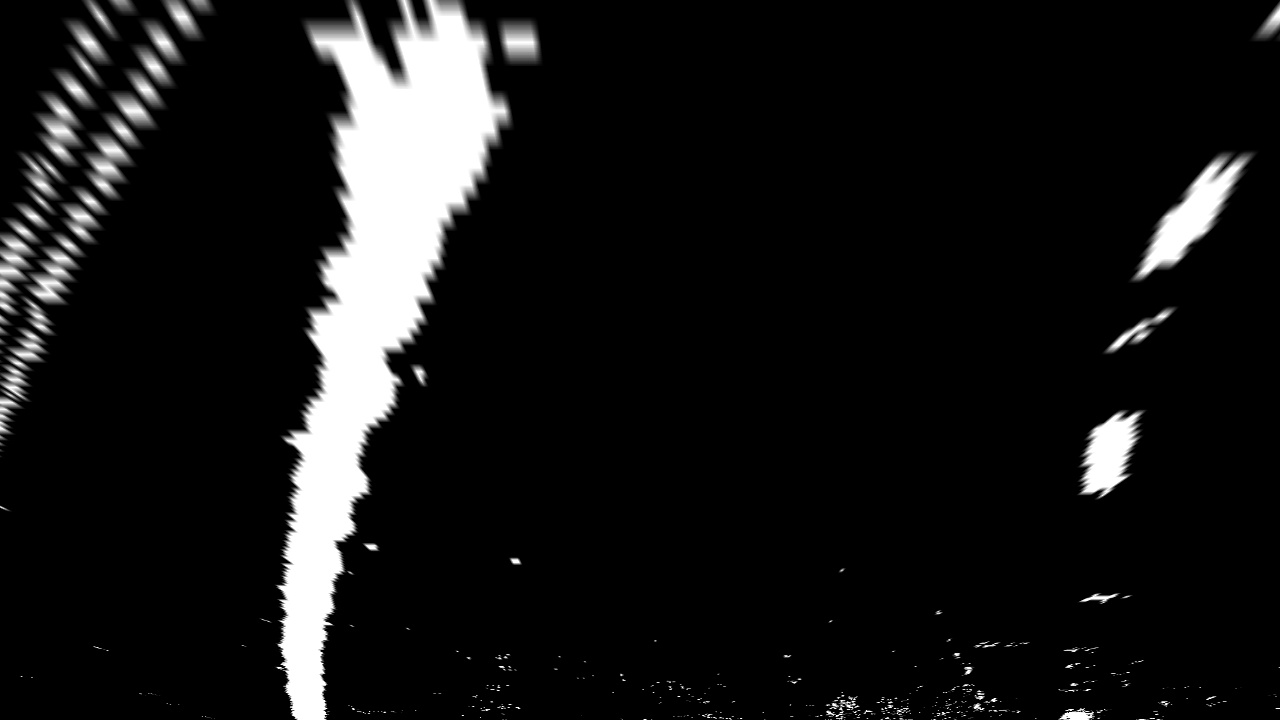
\includegraphics{./output_images/warped_test1.jpg}

\hypertarget{describe-how-and-identify-where-in-your-code-you-identified-lane-line-pixels-and-fit-their-positions-with-a-polynomial}{%
\paragraph{4. Describe how (and identify where in your code) you
identified lane-line pixels and fit their positions with a
polynomial?}\label{describe-how-and-identify-where-in-your-code-you-identified-lane-line-pixels-and-fit-their-positions-with-a-polynomial}}

The sliding windows technique was used to identify lane-line pixels. The
``tracker'' class in the third code cell was used to find the window
centroids. This allowed the lane-lines to be detected and highlighted.
The lanes were marked on the warped images and saved with prefix
``lanes\_''. Here's an example:
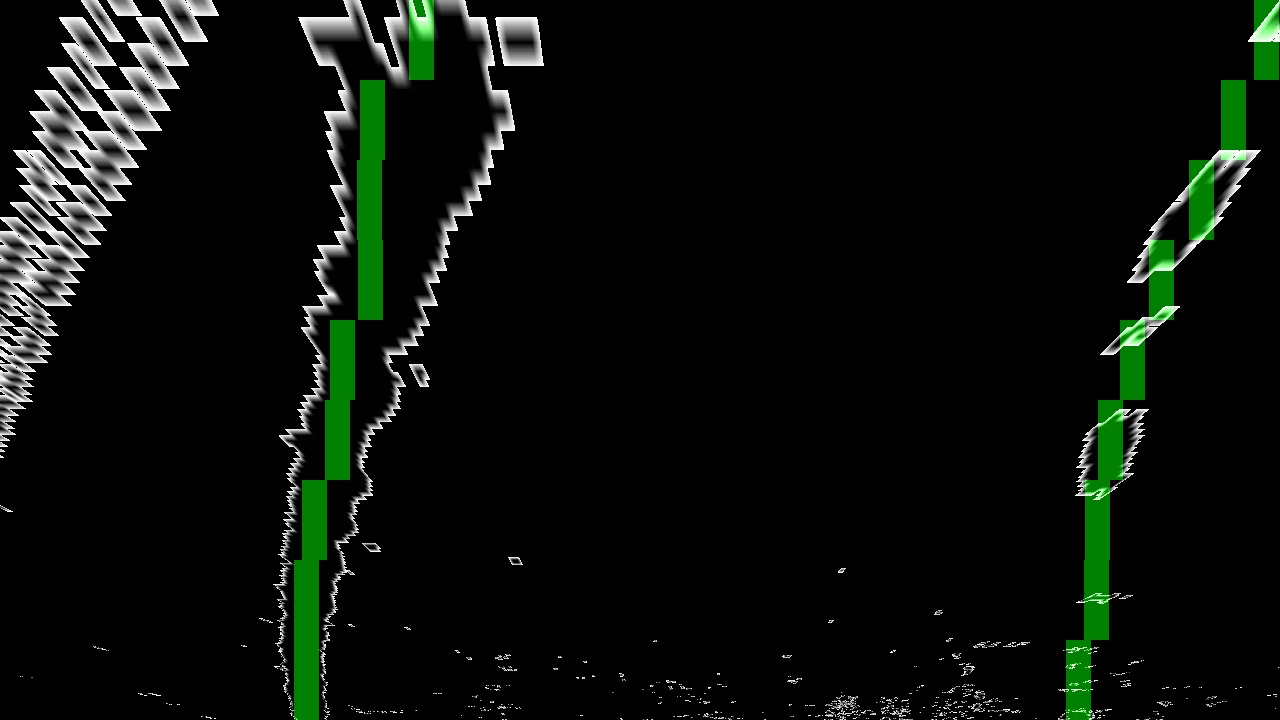
\includegraphics{./output_images/lanes_test1.jpg}

Lane lines polygons were added to the images (red for left and blue for
right) with a middle marker (in green) that defined the area between the
lane lines. The images were unwarped using cv2's warpPerspective with
the inverse transformation matrix to convert it back to a normal view
(from the car). Some color enhancements were made to the image to
emphasize the lane lines. These images were saved with the prefix
``roadwarped\_''. Heres' and example:
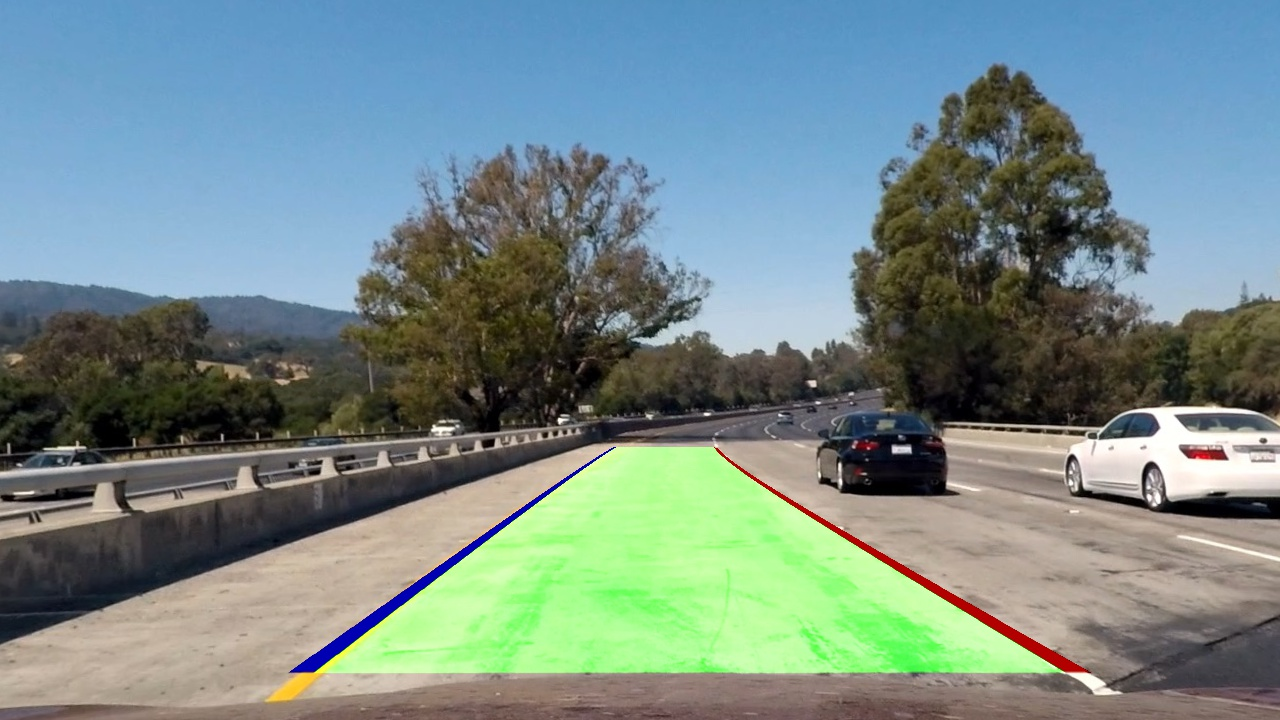
\includegraphics{./output_images/roadwarped_test1.jpg}

\hypertarget{describe-how-and-identify-where-in-your-code-you-calculated-the-radius-of-curvature-of-the-lane-and-the-position-of-the-vehicle-with-respect-to-center.}{%
\paragraph{5. Describe how (and identify where in your code) you
calculated the radius of curvature of the lane and the position of the
vehicle with respect to
center.}\label{describe-how-and-identify-where-in-your-code-you-calculated-the-radius-of-curvature-of-the-lane-and-the-position-of-the-vehicle-with-respect-to-center.}}

The variable curverad is calculated using np.polyfit and the standard
curvature calcuation: curverad = ((1 +
(2\emph{curve\_fit\_cr{[}0{]}}yvals{[}-1{]}\emph{ym\_per\_pix +
curve\_fit\_cr{[}1{]})\textbf{2)}1.5)
/np.absolute(2}curve\_fit\_cr{[}0{]})

The center of the camera's perspective was used as an indication of the
center of the car. This was used to calculate left or right of center.

The radius of curvature and center position of the car were added to the
image as annotation using cv2.putText. Here's an example of a final
annotated image: 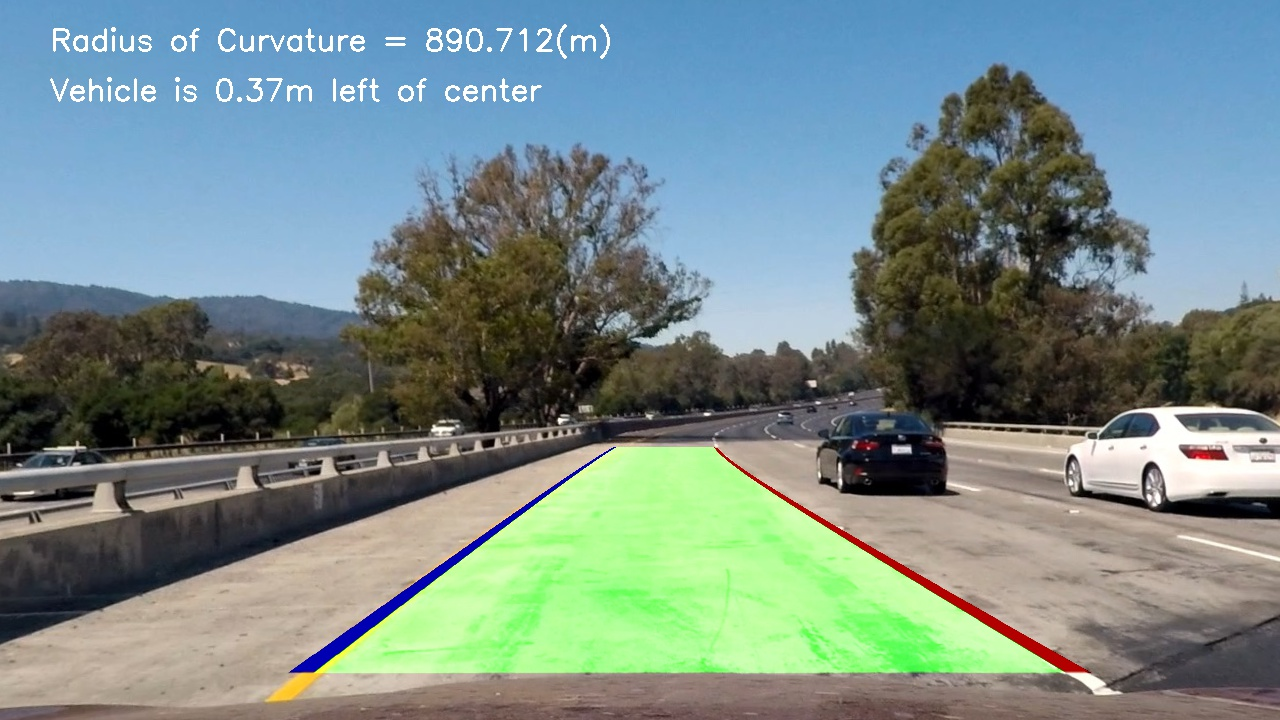
\includegraphics{./output_images/tracked_test1.jpg}

\hypertarget{provide-an-example-image-of-your-result-plotted-back-down-onto-the-road-such-that-the-lane-area-is-identified-clearly.}{%
\paragraph{6. Provide an example image of your result plotted back down
onto the road such that the lane area is identified
clearly.}\label{provide-an-example-image-of-your-result-plotted-back-down-onto-the-road-such-that-the-lane-area-is-identified-clearly.}}

This is the ``roadwarped\_'' image presented earlier. Here it is again:
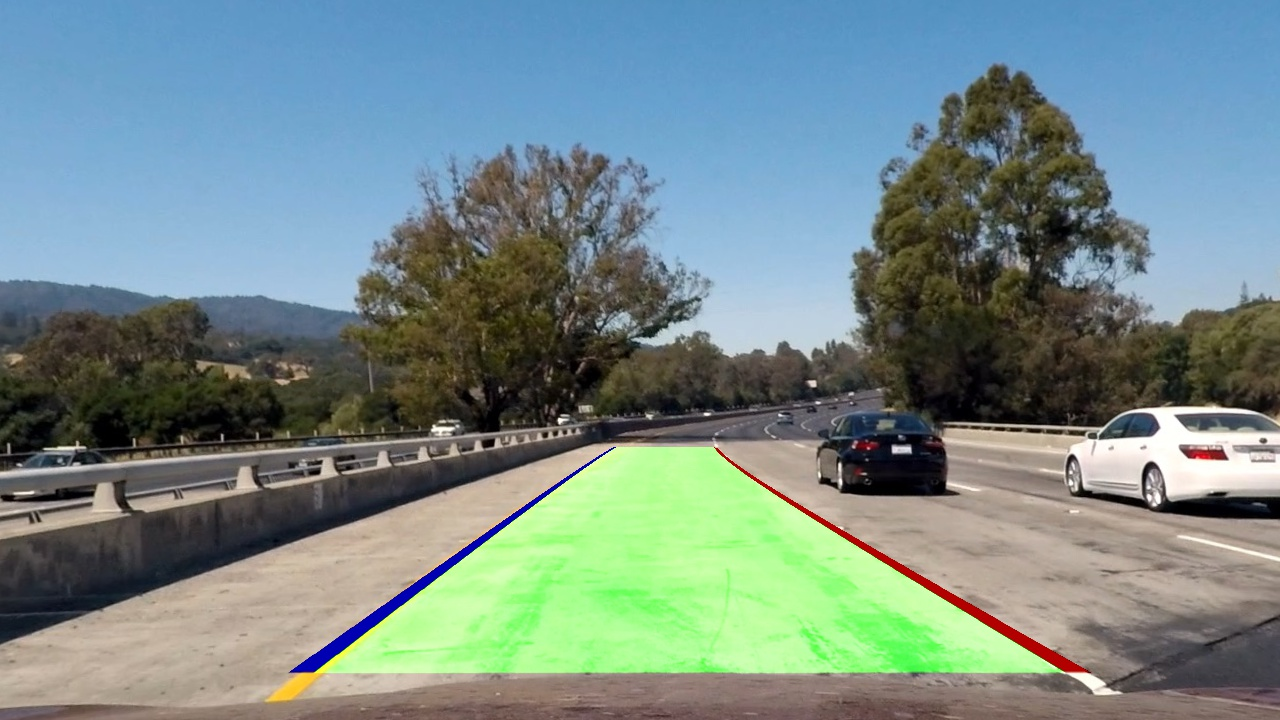
\includegraphics{./output_images/roadwarped_test1.jpg}

\begin{center}\rule{0.5\linewidth}{\linethickness}\end{center}

\hypertarget{pipeline-video}{%
\subsubsection{Pipeline (video)}\label{pipeline-video}}

\hypertarget{provide-a-link-to-your-final-video-output.-your-pipeline-should-perform-reasonably-well-on-the-entire-project-video-wobbly-lines-are-ok-but-no-catastrophic-failures-that-would-cause-the-car-to-drive-off-the-road.}{%
\paragraph{1. Provide a link to your final video output. Your pipeline
should perform reasonably well on the entire project video (wobbly lines
are ok but no catastrophic failures that would cause the car to drive
off the
road!).}\label{provide-a-link-to-your-final-video-output.-your-pipeline-should-perform-reasonably-well-on-the-entire-project-video-wobbly-lines-are-ok-but-no-catastrophic-failures-that-would-cause-the-car-to-drive-off-the-road.}}

I copied the code from the third code cell into the fourth code cell,
creating the function ``process\_image'' by removing the code that read
individual image files along with intermediate image storage to the file
system and returning the final image. Using VideoFileClip from
moviepy.editor, I read the video file and passed it through the
processing, saving it to file ``output1\_tracked.mp4''.

Here's a link to the processed video - \href{./output1_tracked.mp4}{link
to my video result}

\begin{center}\rule{0.5\linewidth}{\linethickness}\end{center}

\hypertarget{discussion}{%
\subsubsection{Discussion}\label{discussion}}

\hypertarget{briefly-discuss-any-problems-issues-you-faced-in-your-implementation-of-this-project.-where-will-your-pipeline-likely-fail-what-could-you-do-to-make-it-more-robust}{%
\paragraph{1. Briefly discuss any problems / issues you faced in your
implementation of this project. Where will your pipeline likely fail?
What could you do to make it more
robust?}\label{briefly-discuss-any-problems-issues-you-faced-in-your-implementation-of-this-project.-where-will-your-pipeline-likely-fail-what-could-you-do-to-make-it-more-robust}}

While coding the project, I found myself referring back to notes and
code examples I had collected while working through the ``class
assignments'' and quizzes. I believe that for the next project, I'll be
more diligent in this area. I found that I didn't fully understand
several concepts (like thresholding and creating the source shape for
transforms). This required additional time while completing the
projecting.

I also noticed that I included virtually no error handling. My lack of
Python knowledge is really hindering me in this area. As I gain more
experience, I'd expect that more error trapping will become common place
in my code.


    % Add a bibliography block to the postdoc
    
    
    
    \end{document}
